\chapter{Decision trees}
\lecture{6}{17/2}

\begin{definition}[Decision tree]
    A \textbf{decision tree} is a tree in which
    \begin{enumerate}
        \item internal nodes represent a \emph{test} on an attribute; 
        \item branches represent the outcome of the test; and
        \item each leaf node represents a \emph{class label}.
    \end{enumerate}
\end{definition}

Decision tree learning is a method commonly used in data mining.
It is a simple representation for classifying examples.

\begin{figure}[]
    \centering
    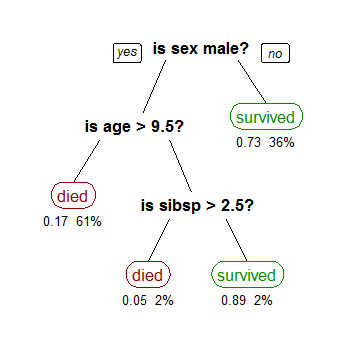
\includegraphics[width=0.8\linewidth]{images/decision-tree}
    \caption{images/decision-tree}%
    \label{fig:decision-tree}
\end{figure}

\begin{example}
    Figure \ref{fig:decision-tree} is an example of a decision tree.
\end{example}

Now let's look at a \emph{metric} for determining how \emph{good} a decision tree is.

\begin{definition}[Gini impurity]
    The \textbf{Gini impurity} is the probability of \emph{incorrectly}
    classifying a randomly chosen element in the dataset if it were
    randomly labelled according to the class distribution in the dataset.
    It is calculated as
    \[
        G = \sum^{C}_{i=1} p_i \, (1 - p_i)
    \]
    where $p_i$ is the probability of randomly picking an element of class $i$
    and $C$ is the number classes.
\end{definition}

\begin{remark}
    As $\sum_{i = 1}^C p_i = 1$ (we have to pick one class), we have
    \[
        G = 1 - \sum_{i=1}^C p_i^2.
    \]
\end{remark}

\begin{example}[Classifying flowers]
    Consider the following decision tree, where a left branch is \emph{true} and a 
    left branch is \emph{false}.
    \begin{center}
        \ttfamily
        \begin{forest}
            [{petal length (cm) <= 2.45}
                [{class = setosa}]
                [{petal width (cm) <= 1.75}
                    [{class = versicolor}]
                    [{class = virginica}]
                ]
            ]
        \end{forest}
    \end{center}
    At each leaf, we can calculate the \emph{Gini impurity} depending on how well
    it classifies our data.
    For example, if $49$ versicolor were correctly identified as versicolor, and 
    only $5$ virginica were incorrectly identified as versicolor (no setosa incorrect
    identified) we have
    \[
        G 
        = \left(\frac{49}{49+5}\right)\left(1 - \frac{49}{49+5}\right)
            + 0
            + \left(\frac{5}{49+5}\right)\left(1 - \frac{5}{49+5}\right)
        = \frac{49}{54} \cdot \frac{5}{54} \cdot 2.
    \]
\end{example}

\begin{definition}[Random forest]
    \textbf{Random forests} are an \emph{ensemble learning} method that operate
    by constructing a multitude of decision trees at training time and then outputting
    the class that is the \emph{mode} of the classes outputted by the different decision trees.
\end{definition}

\begin{remark}
    Random forests (typically) correct decision trees' habit of \emph{overfitting} data to
    their training set.
\end{remark}

The way we construct our decision trees can vary. 
One method is the \emph{random subspace method}:
\begin{enumerate}
    \item first we create a \emph{bootstrapped} dataset which has the
        same size as the original dataset and has randomly selected samples
        (samples can be selected more than once);
    \item we build a decision tree using the \emph{bootstrapped} dataset
        using a random subset of the variables; then
    \item go back to (i) and repeat to preference.
\end{enumerate}
To \emph{use} the random forest, we run our new data through every tree we built
keeping track of the classifications we are given.
We then select the \emph{mode} classification.

\begin{remark}
    Typically, about $\frac13$ of the original data does \emph{not} end up in the
    bootstrapped data.
\end{remark}

\begin{definition}[Out-of-bag error]
    \textbf{Out-of-bag error} (OOB) is a method of measuring the prediction error of
    random forests. 
    OOB is the mean prediction error on each training sample $x_i$, using
    only the trees that did not have $x_i$ in their bootstrap sample.
\end{definition}
